\chapter[Operation of segmented detectors in LN$_{2}$]{Operation of segmented detectors in liquid nitrogen}
\label{cha:GII}
Segmented $n$-type germanium detectors will be directly submerged in cryogenic liquid in GERDA Phase II. It is therefore very important to study the performance of segmented detectors in cryogenic liquid. Siegfried~II,  the second 18-fold segmented $n$-type prototype detector built (see Sec.~\ref{sec:gerda:stat3}), was inserted into the Gerdanlinchen II test stand (see Sec.~\ref{sec:tt:gii}) containing liquid nitrogen on April 23rd, 2008. It was kept in liquid nitrogen for about 5 months and was warmed up on September 15th, 2008. The resolutions and leakage currents of the core and all segments were constantly monitored. Four short cool-down and warm-up cycles were carried out afterward to optimize the setup and perform dedicated measurements. The leakage currents were remeasured after each cool-down. The detector performance is summarized in this chapter.


\section{Experimental setup}
\label{sec:gii:setup}
The measurements were performed using the cryogenic test stand, Gerdalinchen~II (GII). A detailed description of GII can be found in Sec.~\ref{sec:tt:gii}. Figure~\ref{fig:ii:sch} depicts the test stand with three segmented detectors mounted inside. Only the upper and middle detector positions were occupied during the measurements. The dewar is filled bottom up through a filling tube. The numbers inside parentheses indicate the positions of eight PT100 thermal resistors. They were used to monitor the level of the liquid nitrogen. Liquid nitrogen was added once per day to keep its level between PT100 (2) and (3). This ensured that the infrared shields were always kept inside the liquid nitrogen minimizing the infrared radiation load on the detector. 

\begin{figure}[hbtp]
\centering
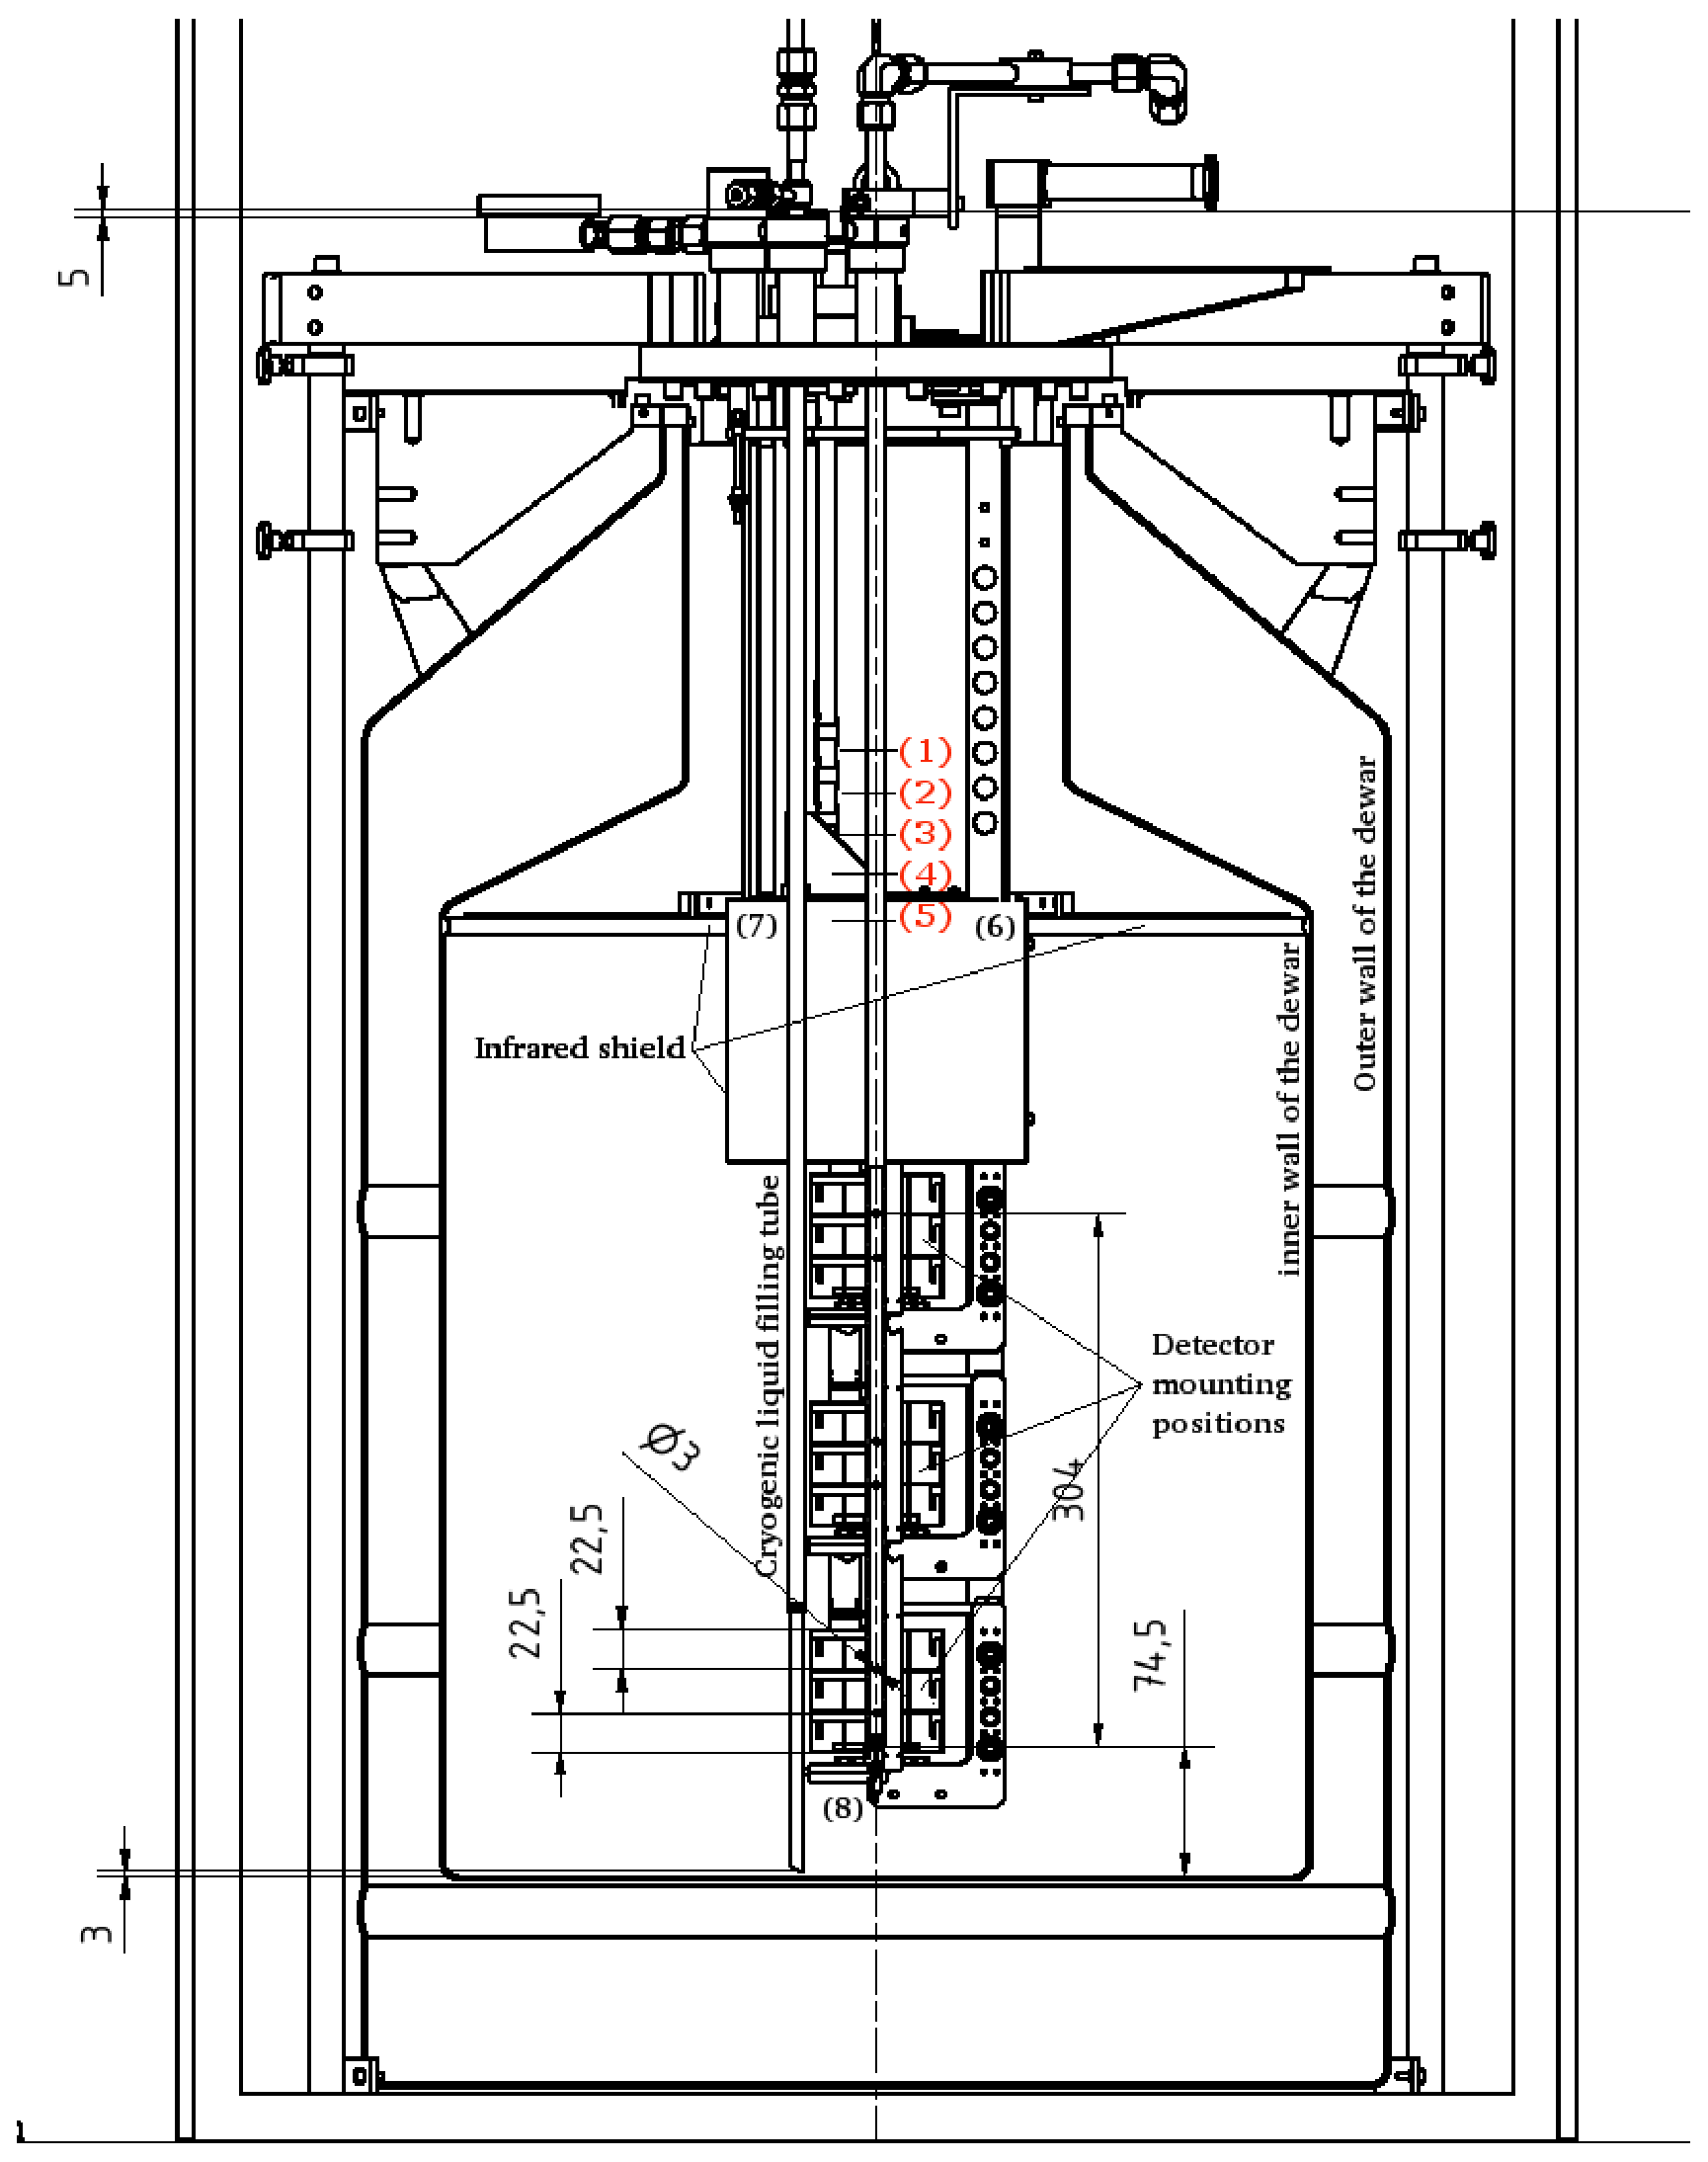
\includegraphics[width=\textwidth]{GIIscheme}
\caption{Gerdalinchen~II setup to operate segmented detectors in liquid nitrogen. For details see text.}
\label{fig:ii:sch}
\end{figure}

\section{Cool-down test}
\label{sec:ii:cool}
The speed, at which the detector strings will be lowered in GERDA, has to be chosen such, that the whole process can be finished in a reasonable time without subjecting the strings and detectors to dangerous thermal and mechanical stress. The submersion speed envisioned for GERDA is 10~mm/min. The temperature profile of a detector during the submersion process was studied in GII with an aluminum mock-up detector mounted at the highest GII position. 

The rising of the liquid nitrogen level was tuned to  about 10~mm/min. The temperature profile of the mock-up detector was monitored using three PT100 thermal resisters mounted on the top, bottom and in the middle of the mock-up. Figure~\ref{fig:ii:temp} shows the temperature profiles of the mock-up detector during the filling of GII. In addition it shows the temperatures measured by the thermal sensor 8 near the bottom of the dewar and the thermal sensor 1 at the top most position always above the liquid. The largest temperature difference between the top and bottom of the detector occurred at the first contact of the detector with the liquid nitrogen. It was about $130^{\circ}$C and lasted about three minutes. While germanium has a thermal conductivity four times smaller than aluminum at room temperatures, the thermal conductivities of germanium and aluminum are almost equal at 80\,K. Thus, it is expected that the germanium detector will cool down at about the same rate as the aluminum mock-up.

\begin{figure}[htbp]
\centering
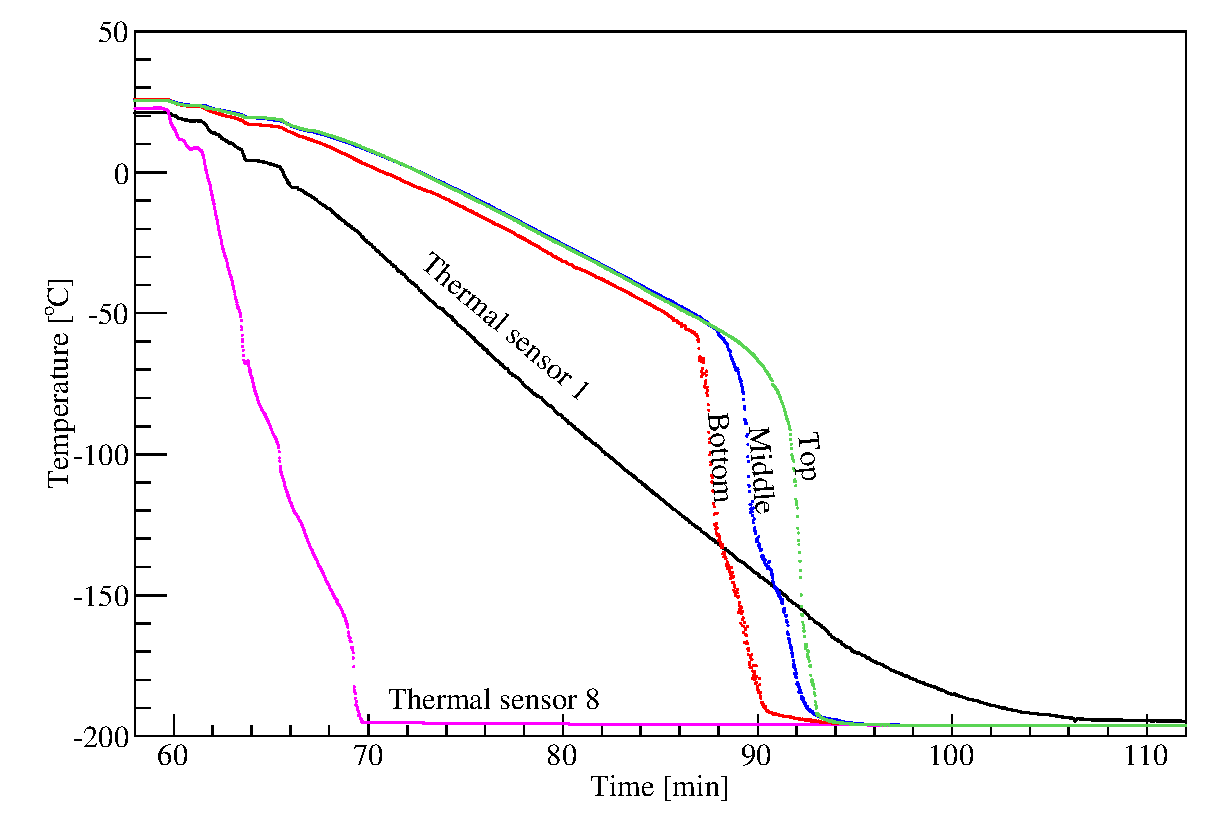
\includegraphics[width=0.8\textwidth]{temp}
\caption{Temperature profile of a mock-up detector during the cool-down process. Curves are shown for sensors mounted on top, middle and bottom of the detector. Also shown are curves for sensors 8 and 1 mounted close to the bottom and top of the dewar.}
\label{fig:ii:temp}
\end{figure}

\section{Resolution}
\label{sec:ii:sigma}
Siegfried II was mounted at the highest position in GII after a detailed cool-down procedure had been developed. It was cooled down on April 23$^{\text{rd}}$, 2008. The core and segment resolutions of Siegfried II were constantly monitored during the 140 days of operation. The variation of the resolutions (FWHM) at 1332~keV is shown for the core in Fig.~\ref{fig:ii:fwhm_core} and for all 18 segments in Fig.~\ref{fig:ii:fwhm_segs}.
\begin{figure}[hbtp]
\centering
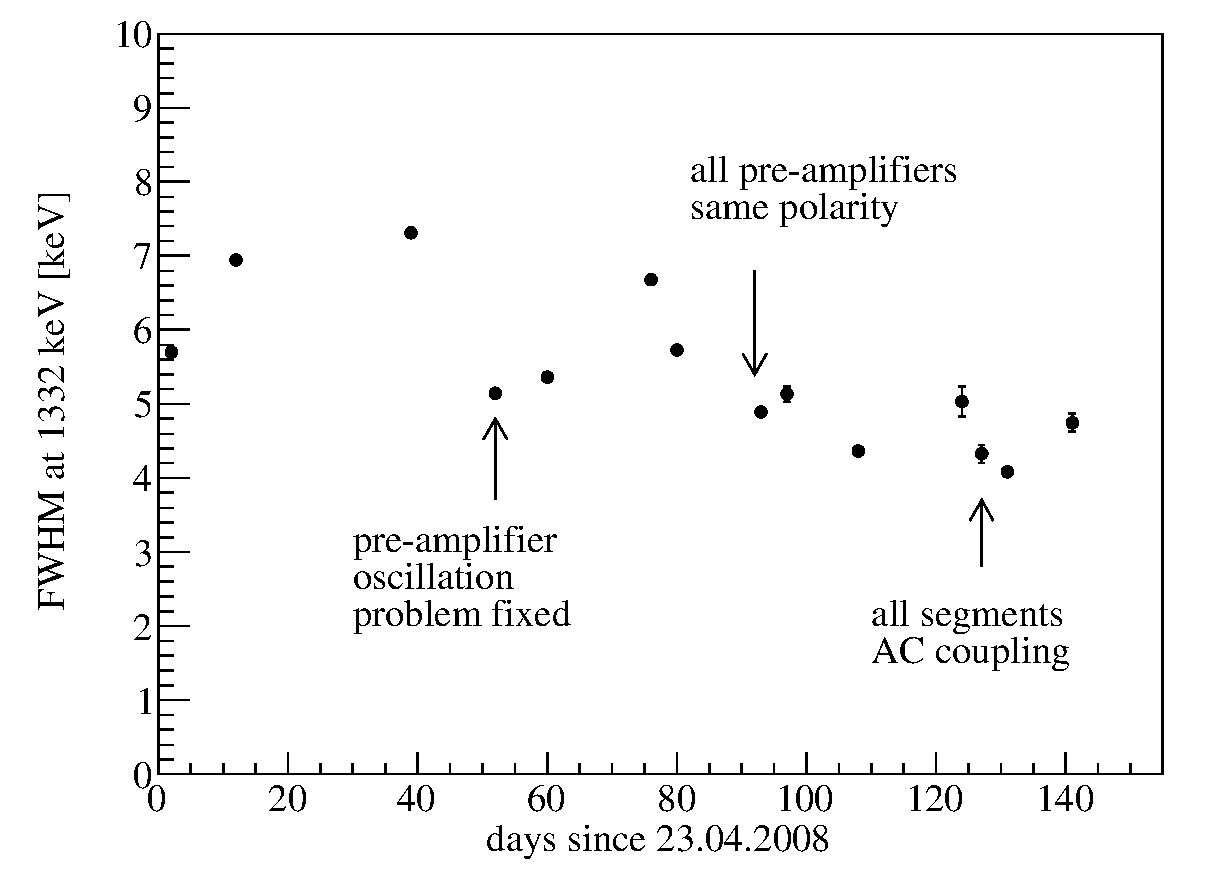
\includegraphics[width=0.6\textwidth]{fwhm_versus_time_core}
\caption{Core resolution of Siegfried II during 140 days of operation as determined from fits to the 1332~keV gamma line. The uncertainties on most values are hidden by the size of the dots.}
\label{fig:ii:fwhm_core}
\end{figure}

\begin{sidewaysfigure}[tphb]
\centering
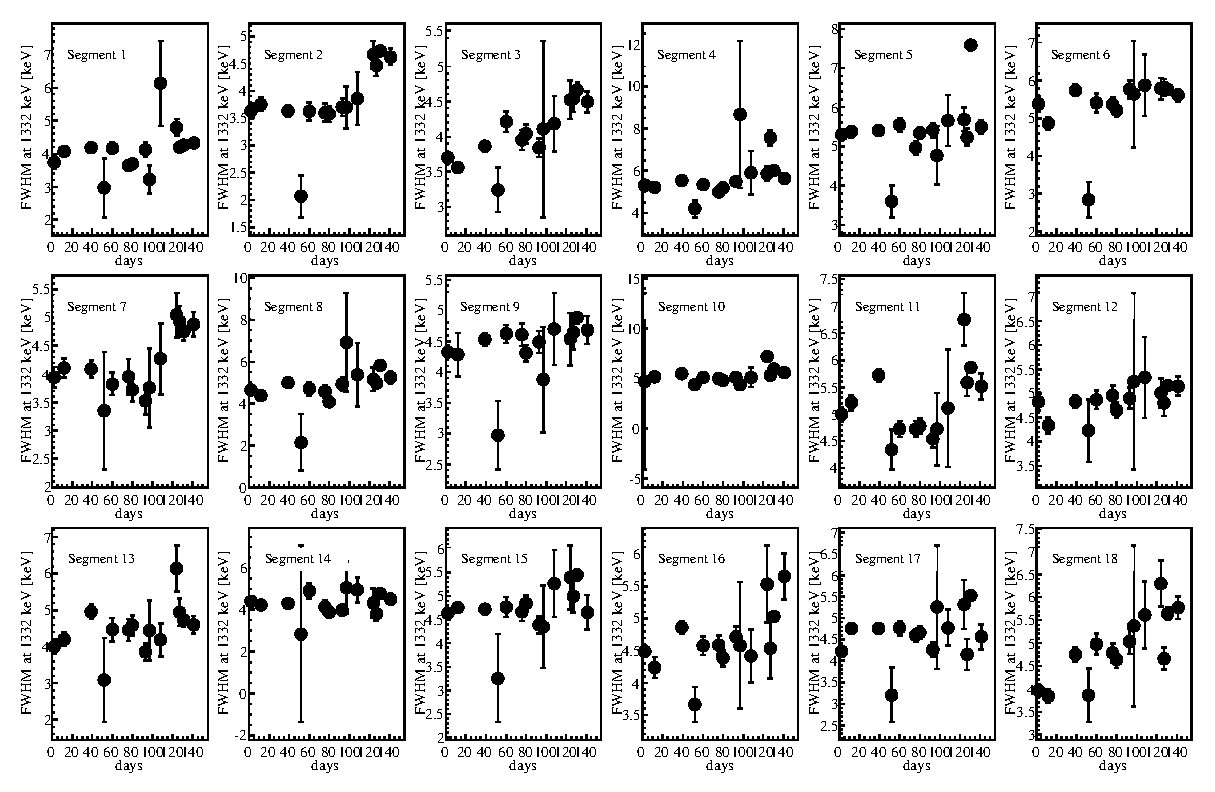
\includegraphics{fwhm_versus_time_segments}
\caption{Segment resolutions of Siegfried II during 140 days of operation as determined from fits to the 1332~keV gamma line.}
\label{fig:ii:fwhm_segs}
\end{sidewaysfigure}

During the first month of operation, all pre-amplifiers were oscillating whenever all 19 channels were read out simultaneously. The oscillations were due to an insufficient grounding scheme for the copper boxes holding and shielding the pre-amplifiers, see Fig.~\ref{fig:tt:gefb}. The problem was fixed by adding an extra copper plate inside the box, serving as the common ground for all pre-amplifiers. Afterward, all pre-amplifiers could be read out simultaneously and the core resolution was slightly better.

The second problem which affected the core resolution was related to the pulse polarity of the pre-amplifiers. Three pre-amplifiers (segments 3, 15 and 17) had a negative signal polarity while the rest had a positive one. This induced cross talk between these three pre-amplifiers and the core pre-amplifier. 
As a result the energy measured by the core for the 1332~keV photon line was 2~keV too low, if the energy was deposited in one of these three segments. These three pre-amplifiers were then replaced, resulting in some improvement in the core resolution as indicated in Fig.~\ref{fig:ii:fwhm_core}.

In order to decouple the segment potentials from the pre-amplifiers, all segment were AC instead of DC coupled ten days before the first warm-up, using 1~G$\Omega$ resistors and 2.2~nF capacitors. This neither influenced the core or segment resolutions.


\section{Leakage current}
\label{sec:ii:current}
The leakage current of Siegfried~II at 2000~V was monitored during the 140 days of operation. Two measurement methods were used: (a) a direct measurement using a picoameter and (b) an indirect measurement comparing the baselines at 0~V and 2000~V. The results from both methods are shown in Fig.~\ref{fig:ii:lc}. The leakage current stayed constant, around 20~pA.

\begin{figure}[htbp]
\centering
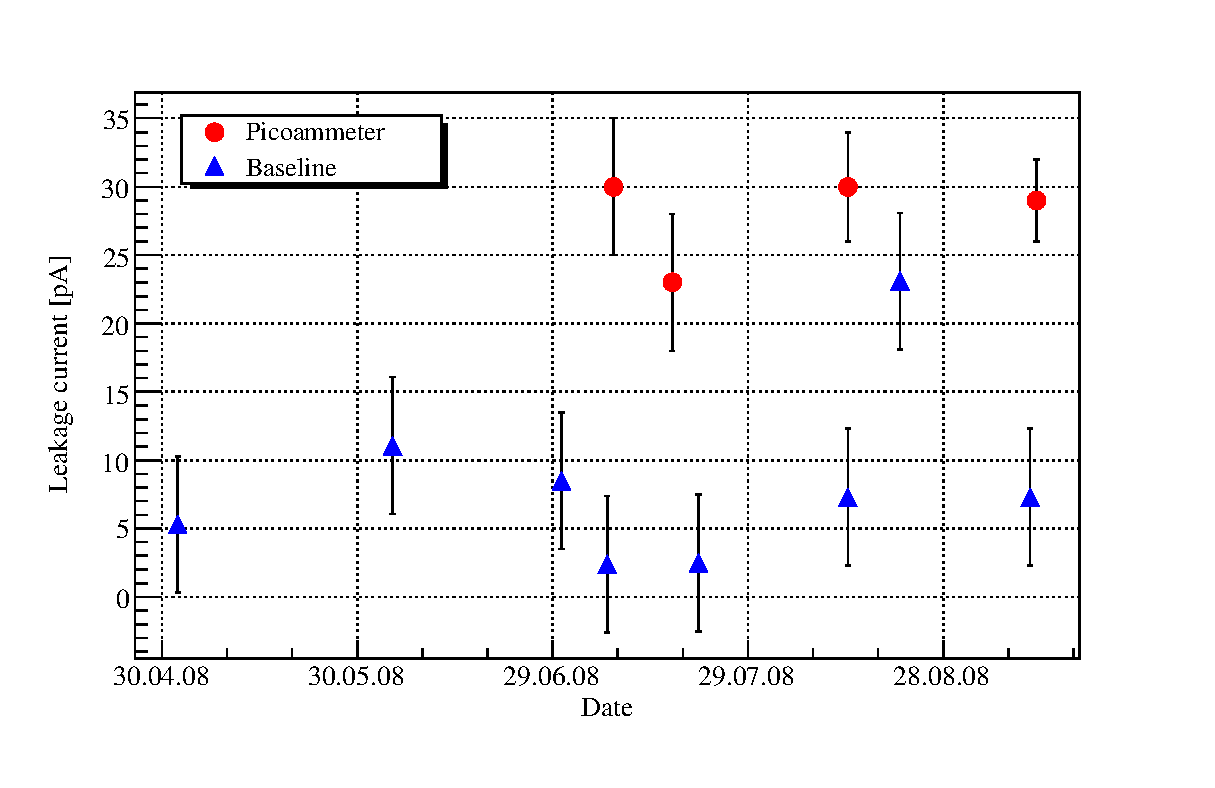
\includegraphics[width=0.6\textwidth, clip]{LC}
\caption{Leakage current of Siegfried II at 2000~V. The results from measurements using a picoameter(dots) and baseline shifts(triangles) are given.}
\label{fig:ii:lc}
\end{figure}

Siegfried~I was added to the setup  at the middle position in GII after the first warm-up of Siegfried~II. Afterward, four cool-down and warm-up cycles were performed. The leakage currents of both detectors at operational voltage after each cool-down are shown in Fig.~\ref{fig:ii:lcs1} and \ref{fig:ii:lcs2}, respectively. The current measured for Siegfried~I showed a significant increase after the third cool-down. This detector had previously been used to test HV contacts in the core and had to undergo reprocessing; it is known to have an imperfect core contact. The currents, measured for Siegfried~II immediately after each cool-down showed  dramatic increases. However, within 40~minutes they dropped back to their original value. Later investigation revealed an increasingly bad segment contact which could account for the effect.

\begin{figure}[htbp]
\centering
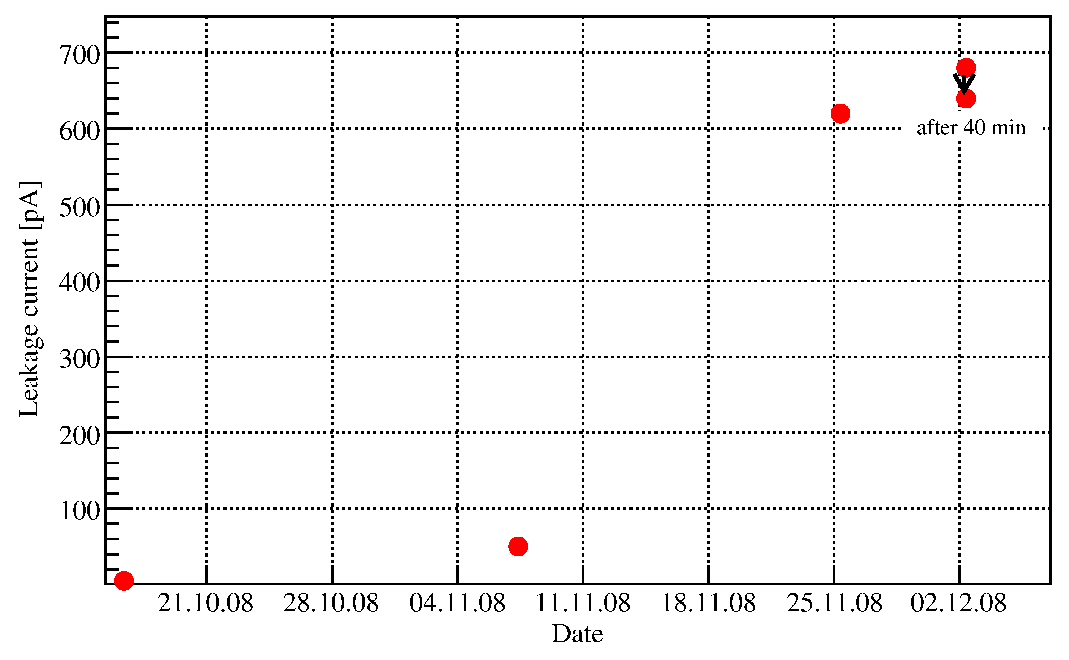
\includegraphics[width=0.6\textwidth]{LCs1}
\caption{Leakage current of Siegfried I at 3000~V right after each cool-down. The currents were measured using a picoameter.}
\label{fig:ii:lcs1}
\end{figure}

\begin{figure}[htbp]
\centering
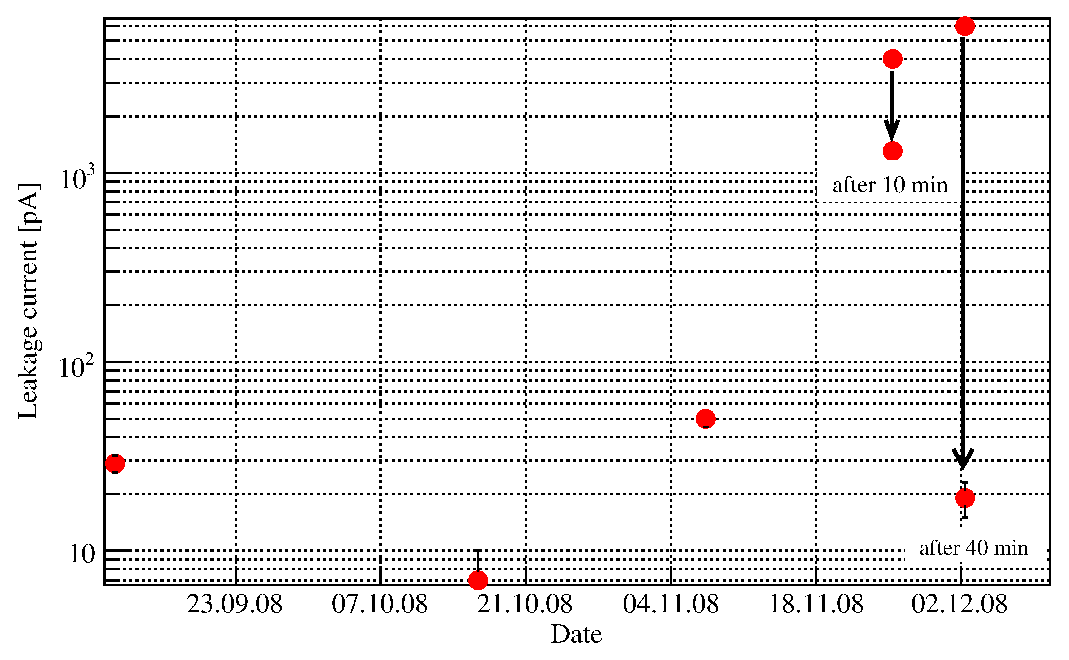
\includegraphics[width=0.6\textwidth, clip]{LCs2}
\caption{Leakage current of Siegfried II at 2000~V after each cool-down. The currents were measured using a picoameter.}
\label{fig:ii:lcs2}
\end{figure}

\section{Summary}
\label{sec:ii:sum}

The 18-fold segmented detector Siegfried~II was operated in liquid nitrogen for four months. No degradation of the performance was observed. Both the Siegfried~I and II detectors underwent four cooling cycles. It was observed that both the core and segment contacts are sensitive to the stress of such cycles. Especially the segment cables should be exchanged after multiple cool-downs.


%%% Local Variables:
%%% mode:latex
%%% TeX-master: "thesis"
%%% End:
